\section{Implementation and computational illustration}\label{sec:computation}

The experiments in this section test whether the predicted grid sizes appear
in practice and whether the certificates are cheap enough to check. They are
not a benchmark of competitive performance: the implementation is a reference
code in exact rational arithmetic, and the instance families are small and
partly designed.

\subsection{Implementation}
The reference implementation is written in Python with exact rational
arithmetic (\texttt{fractions.Fraction}); floating-point input is rejected. It
handles explicit box QPs $c+b^\T x+\frac12x^\T Ax$ with continuous and integer
coordinates, supplied or heuristically computed (minimum-fill) tree
decompositions with arbitrary branching, and empty separators. It implements
the corrected grids of Section~\ref{sec:grids} with per-coordinate corrections
$\max\{A_{ii},0\}w^2/8$, two endpoint labels for coordinates with $A_{ii}\le0$,
two-pass dynamic programming with all min-marginals, the filtering step, and the
capped trials of Algorithm~2. It differs from the analysis in three ways. It
uses a common mesh $h_j=s2^{-j}$ in all coordinates, which is the variant
analyzed with the Euclidean condition number $\kappa$ after
Lemma~\ref{lem:states}, with the larger cap $100\theta^{-1}\lceil\log_2(n+2)\rceil$;
it restarts each trial at the current incumbent rather than at $\ell$, which
the rate analysis allows but our bit-length analysis does not cover; and it
improves incumbents by two sweeps of exact coordinate descent and an optional
convex presolve. None of these affects validity. An exact-output wrapper
implements the acceptance rule of Proposition~\ref{prop:accept} with
stationary-face candidates.

Certificates store the grids, the directed messages and the filtering
decisions of every stage, which is more than Theorem~\ref{thm:certificate}
requires. A separate checker validates the decomposition, recomputes every
table and message, checks every exclusion and the incumbent values, and never
calls the grid generator, the dynamic program or the filtering code of the
solver; it shares only model parsing and objective evaluation. The checker is
independently written, not formally verified. Further modules implement exact
linear and convex box-QP oracles with primal, dual or Farkas witnesses, affine
recourse recognition and lifting, minimum-cut and convex value-factor
recourse, the TU-constrained grids, the endpoint optimal-set descriptor and
explicit polynomial factors, each with its own checker. Code, inputs, raw
results and a one-command reproduction script accompany the paper.

All runs below used one thread per process and at most four processes on an
Intel Xeon w5-2565X under WSL2, Python~3.13, shared with unrelated long-running
jobs (load average 11--16). Timings are single measurements and indicative
only. Every certificate produced in this section was replayed by the checker,
and every replay was valid.

\subsection{Accuracy independence, conditioning and dimension}
The first family has planted nonconvex quadratics on $[-1,1]^n$ with
Hessian $2I+C$, where $C$ has path, random-tree or band sparsity. About a
quarter of the coordinates are at a bound at the planted minimizer $x^*$ and
have a strictly inward gradient; on the others the Hessian block has a
prescribed smallest eigenvalue, and the full Hessian is indefinite. Rational
certificates give $\kappa$ to within 11\%. The family is benign in one respect:
a quadratic minorant certifies $x^*$, which the grid solver does not use.

\begin{figure}[t]
\centering
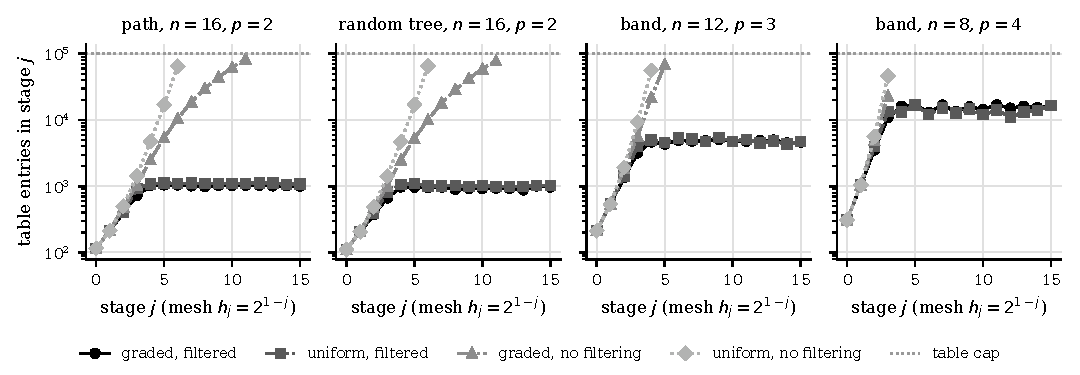
\includegraphics[width=\textwidth]{figures/E1_states_vs_stage.pdf}
\caption{Bag-table states per stage against the stage index $j$ (mesh
$h_j=2^{1-j}$), median of three seeds, for geometric and uniform grids with and
without filtering; $\theta=1/8$, $\kappa\approx4.4$. Unfiltered runs stop at the
table cap of $10^5$ states per stage.}\label{fig:E1}
\end{figure}

Figure~\ref{fig:E1} shows the effect of filtering. On the path with $n=16$,
filtered geometric grids use about $1{,}000$ states per stage from stage~5 to
stage~15, while unfiltered geometric grids reach $83{,}161$ states at stage 11
and unfiltered uniform grids $64{,}879$ at stage 6, after which both hit the cap.
Filtered uniform grids also plateau (about $1{,}090$ states): filtering, not the
grading, removes the dependence on the accuracy, as
Theorem~\ref{thm:cells} predicts. In all theorem-compliant runs the measured
quantities stayed far below the bounds of the analysis: the gap $D(y_j)$ was
at most $0.16\,Lnh_j^2$, the retained radius at most $0.12$ of its bound, and
the number of labels per coordinate at most $0.4\%$ of the cap.

\begin{figure}[t]
\centering
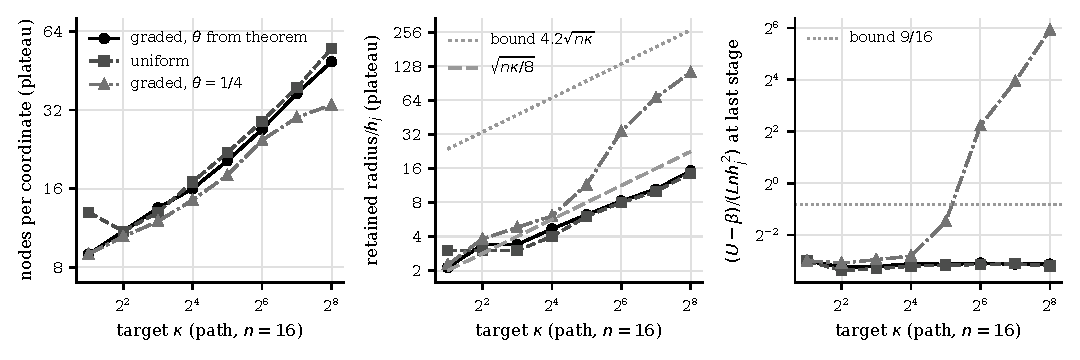
\includegraphics[width=\textwidth]{figures/E2_plateau_vs_kappa.pdf}
\caption{Path with $n=16$ and target $\kappa=2,\dots,256$. Left: labels per
coordinate at the plateau. Middle: retained radius over $h$, with the bound
$5\sqrt{n\kappa}$ and the reference $\sqrt{n\kappa}$. Right: last-stage gap over
$Lnh^2$; with the fixed grading $\theta=1/4$, which violates
$8\kappa\theta^2\le1$, contraction fails for $\kappa\ge64$.}\label{fig:E2}
\end{figure}

Figure~\ref{fig:E2} varies $\kappa$ on the path. The plateau grows from 9 to 49
labels per coordinate with the grading prescribed by the theorem, and the
retained radius grows like $\sqrt\kappa$ and stays far below its bound. With the
fixed grading $\theta=1/4$ the condition $8\kappa\theta^2\le1$ fails for every
instance; the method still contracted for $\kappa\le32$, but for $\kappa\ge64$ the
last-stage gap divided by $Lnh^2$ was $4.7$, $15$ and $61$. The capped schedule
handled this automatically: it succeeded in its first trial for $\kappa\le32$ and
restarted once or twice for larger $\kappa$, earlier than the theorem guarantees.
On paths with $n=4,\dots,128$ and $\kappa\approx2$, filtered uniform grids used
exactly $4(\lfloor\sqrt{n/4}\rfloor+1)+1$ labels, the $\sqrt n$ law of
Proposition~\ref{prop:tu-tight}, while graded grids grew from 9 to 19 labels;
this range of $n$ is too small to separate $\log n$ from $\sqrt n$ cleanly.

\subsection{The expanding-box chain}
Table~\ref{tab:chain} reports the family $G_m$ of Example~\ref{ex:chain} for
target gap $10^{-3}$. The largest coordinate grid grows from 5 to 11 nodes as
$n$ grows from 4 to 128, the number of stages grows linearly in $m$ because the
box widths are $2^t$, and all runs succeeded in the first trial. The exact
Bellman message for $S_m$ would need at least $2^{m-1}$ quadratic pieces
(Proposition~\ref{lim:prop:messages}).

\begin{table}[t]
\centering
\caption{Certified approximation of the expanding-box chain $G_m$ (gap
$\le10^{-3}$). ``Nodes'' is the largest number of nodes of a coordinate grid,
``states'' the total number of bag-table states, and the last column the lower
bound on the number of pieces of an exact message.}\label{tab:chain}
\begin{tabular}{rrrrrrrr}
\toprule
$m$ & $n$ & stages & nodes & states & solve (s) & replay (s) & message pieces\\
\midrule
2 & 4 & 9 & 5 & 808 & 0.01 & 0.02 & $\ge2$\\
4 & 8 & 12 & 6 & 3{,}143 & 0.06 & 0.10 & $\ge8$\\
8 & 16 & 16 & 8 & 9{,}403 & 0.16 & 0.29 & $\ge128$\\
16 & 32 & 25 & 9 & 36{,}123 & 0.76 & 1.28 & $\ge3.3\cdot10^4$\\
32 & 64 & 41 & 10 & 153{,}981 & 3.50 & 6.21 & $\ge2.1\cdot10^9$\\
64 & 128 & 74 & 11 & 585{,}760 & 14.8 & 28.7 & $\ge9.2\cdot10^{18}$\\
\bottomrule
\end{tabular}
\end{table}

\subsection{Exact output}
Twenty small instances were solved exactly: twelve random unplanted
mixed-integer QPs ($n=3,\dots,6$), three with two isolated minimizers, three
planted instances and two with a segment of minimizers. An independent
enumeration of integer labels and continuous faces gives the reference
optima. Exact output was certified for 18 instances, all with the correct value
and an optimal point. The number of stages tracked the number of bits that the
acceptance rule requires: at most one stage for three instances with $n=3$,
67--144 stages for 49--120 bits on the other random and tied instances, and 275
and 534 stages for 208 and 342 bits on the planted ones. The two instances with
a segment of minimizers stopped at the 5-second limit with certified gaps of
about $2^{-11}$, against about $2^{-53}$ required; this is the behaviour
expected without growth, where only finite termination is guaranteed
(Theorem~\ref{thm:exact}).

\subsection{Comparison with a global solver}
Table~\ref{tab:scip} compares the reference implementation with SCIP~10.0
\cite{VigerskeGleixner2018,BestuzhevaEtAl2023} on the planted family with $\kappa\approx4.4$, three seeds
per row. SCIP ran single-threaded on the epigraph formulation
$\min\{t:t\ge F(x)\}$ with absolute gap $10^{-6}$ and a 20-second limit; the
certified solver used the capped schedule with $\varepsilon=10^{-6}$. SCIP
reached its gap on the instances with $n\le16$ and hit the time limit on all
paths with $n\ge32$. The certified solver reached a replayed gap below $10^{-6}$
on all 21 instances. SCIP's incumbents were optimal to about $10^{-14}$ when
evaluated exactly, and its dual bounds were valid, but every reported SCIP
primal bound lay below the true optimum, by $1.8\cdot10^{-6}$ to
$1.6\cdot10^{-5}$, because the epigraph constraint is satisfied only within its
feasibility tolerance. This is the usual behaviour of floating-point solvers
and the reason a separate exact check is useful. The comparison uses one
formulation, default settings and a family that favours decompositions of
small width; it is not a performance ranking.

\begin{table}[t]
\centering
\caption{Planted family, $\kappa\approx4.4$, three seeds per row: maximum solve and
replay times of the certified solver (gap $\le10^{-6}$, all certified) and SCIP
status and maximum time (20-second limit). ``Bag'' is the maximum bag
size.}\label{tab:scip}
\begin{tabular}{lrrrrll}
\toprule
graph & $n$ & bag & solve (s) & replay (s) & SCIP status & SCIP (s)\\
\midrule
path & 16 & 2 & 0.36 & 0.39 & gap reached & 5.4\\
tree & 16 & 2 & 0.39 & 0.43 & gap reached & 0.7\\
band & 12 & 3 & 1.38 & 2.07 & gap reached & 1.4\\
band & 8 & 4 & 6.60 & 11.5 & gap reached & 0.3\\
path & 32 & 2 & 1.01 & 1.06 & time limit & 20\\
path & 64 & 2 & 2.64 & 3.50 & time limit & 20\\
path & 128 & 2 & 6.87 & 9.85 & time limit & 20\\
\bottomrule
\end{tabular}
\end{table}

\subsection{Recourse}
Table~\ref{tab:recourse} compares plain corrected grids with the recourse
pipeline on six fixed diagnostic instances, at target gap $2^{-10}$ and a
20-second limit. The affine stars have a concave core coordinate and 4 or 16
leaves coupled to it by stiff convex squares $64(y_i-x_0/2)^2$, with variables
in random order; recognition finds the globally affine responses and the
reduced problem is solved exactly. The piecewise instances are the family of
Example~\ref{ex:cv-fm} with $M=1$ and $M=100$; the certified convex value
factor removes the dependence on $M$. The dense instances have one convex
core coordinate and a residual that is concave in each coordinate and
submodular, with a complete interaction graph; the minimum-cut oracle of
Section~\ref{sec:cuts} replaces a decomposition of bag size $n$. All
certificates were replayed by the respective checkers. These are designed
examples of the structures in Section~\ref{sec:recourse}, not hard instances.

\begin{table}[t]
\centering
\caption{Plain corrected grids versus recourse (gap target $2^{-10}$, 20-second
limit). ``States'' counts bag-table states of the plain grid runs; times in
seconds, solve and replay.}\label{tab:recourse}
\begin{tabular}{lrrlrrrlrr}
\toprule
&&&\multicolumn{4}{c}{plain grids}&\multicolumn{3}{c}{recourse}\\
\cmidrule(lr){4-7}\cmidrule(lr){8-10}
instance & $n$ & bag & status & gap & states & solve & status & solve & replay\\
\midrule
affine star & 5 & 2 & time limit & 0.019 & 559{,}320 & 20.0 & exact & 0.005 & 0.001\\
affine star & 17 & 2 & time limit & 1.23 & 823{,}569 & 20.0 & exact & 0.061 & 0.057\\
piecewise, $M=1$ & 3 & 3 & certified & $4\cdot10^{-4}$ & 498 & 0.017 & certified & 0.013 & 0.003\\
piecewise, $M=100$ & 3 & 3 & certified & $7\cdot10^{-4}$ & 35{,}600 & 0.63 & certified & 0.004 & 0.002\\
dense cut & 7 & 7 & certified & $1\cdot10^{-3}$ & 2{,}038 & 0.044 & exact & 0.003 & 0.003\\
dense cut & 33 & 33 & table limit & 2.96 & 0 & 0.021 & certified & 0.078 & 0.064\\
\bottomrule
\end{tabular}
\end{table}

\subsection{Limits}
The cost of the method is exponential in the bag size, and exact rational
arithmetic dominates the running time; the band with bag size four already
takes several seconds. A first release of the code was also run on two binary
instances from QPLIB \cite{FuriniEtAl2019}, QPLIB\_3852 (231 variables) and QPLIB\_5881 (120 variables).
The best decompositions found by the minimum-fill heuristic have widths 19
and 93, and both runs stopped at the table limit before the first stage,
keeping only the trivial initial bound. Large width, not the accuracy, is the
binding limit of the approach; Section~\ref{sec:limits} shows that this is
unavoidable in the worst case.
